\section{Formal devices}

\frame{
	\frametitle{Directed B-hypergraphs}
	
	A hypergraph $\angbrack{V, E}$ consists of
	\begin{itemize}
		\item a set of nodes $V$
		\item a set of edges $E$
		\item an edge $e$ has 
		\begin{itemize}
			\item a head node $\head(e) \in V$ 
			\item a tail $\tail(e) \in V^*$ (sequence of nodes)
		\end{itemize}
		%\item $BS(v)$ is the set of incoming edges to $v$
	\end{itemize}
	
	\pause
	
	\begin{footnotesize}
	\begin{columns}
	\begin{column}{0.5\textwidth}
	CFGs
	\begin{itemize}%[noitemsep,nolistsep]
		\item nonterminal \ra node
		\item terminal \ra terminal node 
		\item rule \ra edge
		\item LHS \ra head
		\item RHS \ra tail
	\end{itemize}
	\end{column}
	\pause
	\begin{column}{0.5\textwidth}
	FSAs
	\begin{itemize}%[noitemsep,nolistsep]
		\item state \ra node
		\item symbol \ra terminal node
		\item transition \ra edge
		\item origin \ra tail node
		\item destination \ra head
	\end{itemize}
	\end{column}
	
	\end{columns}
	\end{footnotesize}
		
	
}

\frame{
	\frametitle{A forest as a hypergraph}
	
	\begin{center}
	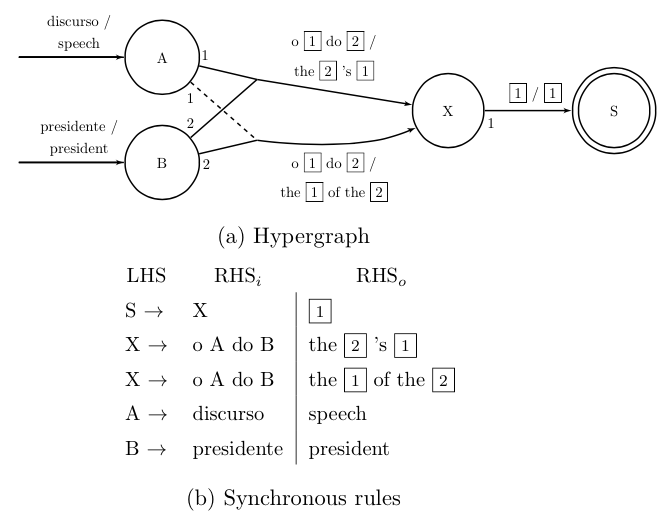
\includegraphics[scale=0.4]{img/hg}
	\end{center}
	
}

\frame{
	\frametitle{Weighted sets}
	
	A weighted set $\angbrack{\mDD, \omega}$ consists of 
	\begin{itemize}
		\item a set of structures (e.g. hyperpaths/derivations)
		\item a function $w : \mDD \ra \mathcal{K}$
	\end{itemize}
	
	~
	
	Let us focus on weighted sets whose weight functions factorise
				$$w(\mdd) = \bigotimes_{e \in \mdd} w(e)$$ 
				
	~
	
	Often the structure is just a means to an end (the yield)
			$$w(\myy) = \bigoplus_{\mdd \in \mDD_\myy} w(\mdd)$$ 
	
}

\frame{
	\frametitle{Semirings}
	
	An algebraic structure $\mathcal{K} = \angbrack{\mathbb{K}, \oplus, \otimes, \bar{0}, \bar{1}}$ \pause
	\begin{itemize}
		\item $\mathbb K$ is a set (e.g. $\mathbb N, \mathbb R, \{0, 1\}$) \pause
		\item $\oplus$ and $\otimes$ are binary operators \pause
		\item $\oplus$ is commutative and has identity $\bar{0}$\\ 
		$a \oplus b = b \oplus a$ and $\bar{0} \oplus a = a \oplus \bar{0} = a$ \pause
		\item $\otimes$ is associative and has identity $\bar{1}$\\
		$(a \otimes b) \otimes c = a \otimes (b \otimes c)$ and $\bar{1} \otimes a = a \otimes{1} = a$ \pause
		\item $\otimes$ left distributes over $\oplus$\\
		$a \otimes (b \oplus c) = (a \otimes b) \oplus (a \otimes c)$ \pause
		\item $\bar{0}$ is the $\otimes$-annihilator \\
		$\bar{0} \otimes a = a \otimes \bar{0} = \bar{0}$
	\end{itemize}
}

\frame{
	\frametitle{Examples of semirings}
	
	
	\begin{center}
	\begin{tabular}{l | c | c | c | c | c}
	Name      & $\mathbb K$ & $\oplus$& $\otimes$& $\bar{0}$ & $\bar{1}$\\ \hline \hline
	\textsc{Binary}    & $\{0, 1\}$  & $\vee $ & $\wedge$ & $0$ & $1$ \\
	\textsc{Counting}  & $\mathbb N$ & $+$     & $\times$ & $0$ & $1$ \\
	\textsc{Prob}      & $[0, 1] \subset \mathbb R$ & $+$     & $\times$ & $0$ & $1$ \\
	\textsc{LogProb}   & $\mathbb R \cup \{-\infty\}$ & $\oplus_{\log}$ & $+$ & $-\infty$ & $0$\\
	\textsc{Viterbi}   & $\mathbb R \cup \{-\infty\}$ & $\max$ & $+$  & $-\infty$ & $0$\\
	\end{tabular}
	\end{center}
	
	~
	
	where $a \oplus_{\log} b = \log(\exp(a) + \exp(b))$
}